% this file is called up by thesis.tex
% content in this file will be fed into the main document

%: ----------------------- name of chapter  -------------------------
\chapter{Problem Solution} % top level followed by section, subsection

In this chapter improvements to the existing implementation are discussed. First, changes in the Arduino sensor module are described. Secondly, an overview of changes in the communication between the module and data collection server (the server from here on). Lastly, an overview of the fuzzy control and data prediction systems that were implemented to reduce communication overhead and power consumption.

The main goal is to reduce the average power consumption measured by \todo{reference it somehow} the PeakTech power supply. 

\todo{introduction}

%: ----------------------- paths to graphics ------------------------

% change according to folder and file names
\ifpdf
    \graphicspath{{X/figures/PNG/}{X/figures/PDF/}{X/figures/}}
\else
    \graphicspath{{X/figures/EPS/}{X/figures/}}
\fi

\section{Power Consumption}

The first problem addressed is power consumption. There are two main ideas behind reducing it - put the sensor module to sleep mode when not transmitting data and reduce the need for data transmission. For this, the server-side client was improved to predict sensor data when possible and notify the sensor module of the next data transmission time. This enables the module to enter sleep mode for the given time period and thus reduce power consumption. 

\subsection{Sleep}

Since the module consists of 3 components - Arduino Mega ADK, Wireless SD Shield with WiFly module and TinkerKit Sensor Shield. Both the Mega ADK and WiFly module support sleep modes. 

\subsubsection{Watchdog Timer}
A watchdog timer \cite{watchdog_timer} is an electronic timer used to recover from computer malfunctions. They are found in automated systems where human interference is not possible and therefore the system must be able to recover from malfunctions on its own. 
A watchdog timer essentially performs a timing function producing a delayed response to an input trigger. The most common implementation has a digital counter that counts from a specified value down to a terminal value. Usually the initial value is programmable. When the counter reaches the terminal value, the timer timeouts and triggers a timeout signal. Usually this means restarting the program from the start. A program can restart the watchdog timer at any time. The act of restarting is usually referred to as "kicking the dog". In this way, a program can be written witch never lets the counter reach the terminal value.

\subsubsection{Arduino Mega ADK}

In case of an Arduino board, when the watchdog timer timeouts, the sketch is restarted (new call to $setup()$). Furthermore, a watchdog timeout signal is sent and this signal can be captured by the sketch. In the Arduino sketch, this is implemented by the JeeLib library \cite{jeelib_general}. JeeLib is a library written for experimenting with JeeLabs products, however, some parts of the library are written for Arduino boards and can be used with them. Specifically, the Ports class \cite{jeelib_port} is the one used in this implementation to put the Arduino Mega ADK into sleep mode. The sketch execution stops for the specified sleep time and afterwards execution continues from the call to sleep function.

\todo{Add a sample overview of the sketch here maybe?}

\subsubsection{WiFly module}

The RN-XV WiFly module can be put to sleep in two ways - sleep timer or sleep command. With the sleep timer, the shield will enter sleep mode after a specified time period has passed since all TCP active connections have closed. With the sleep command the module will enter sleep mode immediately, unless an active TCP connection exists. \cite{wifly_manual}. 

This means that in order to put the WiFly module to sleep, all active connections must be closed. For the XMPP session, this means closing the active stream and the underlying TCP connection. Once this has been done, the module can successfully enter sleep mode. 

The module can be waken up by either sending characters of the UART or by using the wake timer. In our implementation the activity on the UART wakes the module up when the sketch execution continues after the Mega ADK wakes up from sleep mode and establishes a new TCP connection in the start of $loop()$ method call. This effectively means going through the first 5 stages of XMPP session lifecycle on every wake up. 
Since XMPP session initialization is quite verbose and the communication over Wi-Fi is unstable, the possibility of receiving scrambled or incomplete messages creates a problem. 

\subsection{Communication}

Because all TCP connections and therefore the XMPP session have to be closed after every data transmit, XMPP session lifecycle steps 1 - 5 shown in \autoref{xmpp_lifecycle} are executed multiple times. When testing the XMPP implementation with Arduino Mega ADK and WiFly module sleep modes enabled, a troubling fact was discovered - the XMPP session negotiation fails at least once for every 30 minute test. The reason for these connection failures are scrambled authentication or stream opening stanzas. 

From the tests, it could be seen that the average XMPP session start up time was 15 seconds. \todo{show a graph here i guess? or whatever} Data needs to be transmitted every 10 seconds, which means that the module can never be put to sleep as it will not be able to go through the sleep and wake up cycle during the available time period. Moreover, data transmission took on average 1 second, meaning that 15 seconds spent on wake up would result in a second of actual work, which is not efficient. 

During testing the sleep and wake up cycles with XMPP, it was found that XMPP session negotiation will hang approximately once in 15 minutes. As the maximum sleep time in our implementation is 65 seconds, this means that there are at least 13 separate session negotiations. Of course, this is the problem of the XMPP library in use and its lack of error handling. Problems with the library could be addressed with a better implementation, however, there was another factor discovered during the tests.

As a result, XMPP as a means of communication was not viable when trying to minimize power consumption. As an alternative, \todo{look how to reference these} web sockets, raw sockets and HTTP was considered. Web sockets were left out because opening a web socket connection is opened with a HTTP request, making using that one request to actually send the data more efficient. Therefore, HTTP was preferred to web sockets. Raw socket implementation in Arduino would add needless complexity to the sketch and was therefore not implemented. 

The main advantages of HTTP are connection initialization speed and simplicity. The average time to wake up from sleep mode, send an HTTP request and receive response from the server, was measured to be around 5 seconds. In the previous scenario of 10 second transmission interval, it would mean 5 seconds could be spent in sleep mode, 5 seconds to wake up and transmit the data. This implementation would be more energy efficient, which can be seen in \autoref{30s_interval_power}. The data was gathered while running the prototype for 30 minutes with a data sending interval of 30 seconds. The sleep times were adjusted for both configurations based on their wake up times. As seen in the figure, the HTTP configuration consumes approximately 20\% less power than the one using XMPP. 

\todo{Add a sample request here}

\begin{figure}[h]
\centering
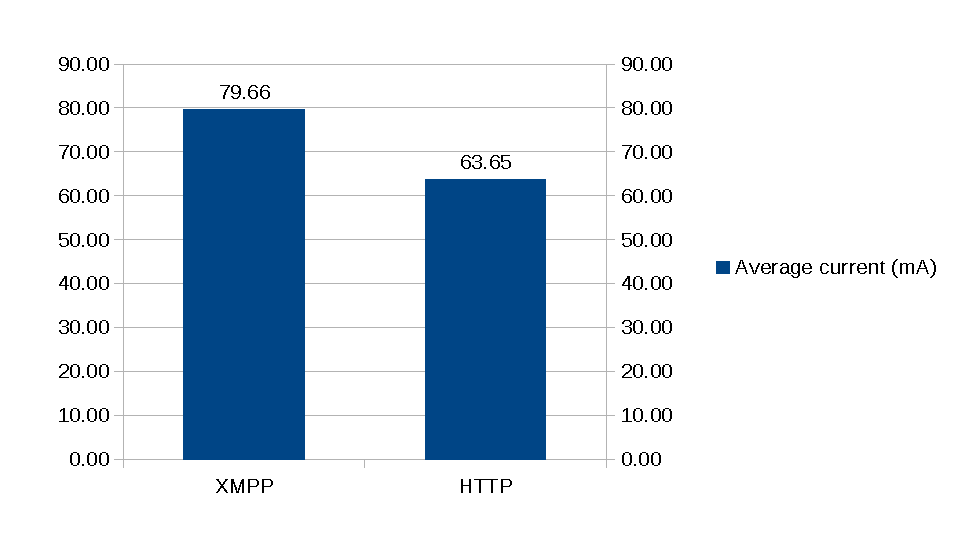
\includegraphics[scale=0.9]{4/figures/30s_xmpp_vs_http.pdf}
\caption{Power Consumption at 30 Second Interval}
\label{30s_interval_power}
\end{figure}

\section{Server-side Client}

With the move from XMPP to HTTP, the server-side client's implementation changed. Instead of using XMPP Smack library, a web server was needed. Jetty was selected because of its simplicity and possibility to embed it into the application. A web server embedded in an application is useful when prototyping, because it saves time on configuration and deployment. 

Furthermore, to take full advantage of the newly developed sleep mode functionality, the client was further developed to predict sensor values for some time. Two modules were added the server for this - simple linear regression and fuzzy control engine. In addition, the data model was modified to suit the new modules. The new data model can be seen in \autoref{data_model_final}. $Data$ table now has $measured$ field, which indicates if the value has been measured or predicted. $SensorTypes$ table has two new fields - $regression\_error$ and $measure\_error$. $regression\_error$ is the acceptable regression model error for future predictions. $measure\_error$ indicates the acceptable variance for measured values. 

\todo{Do i really need this here?}
The final web server consists of 4 modules:
\begin{enumerate}
\item Request handler
\item Linear regression model
\item Fuzzy control engine
\item Data storage
\end{enumerate}

\begin{figure}[h!]
\centering
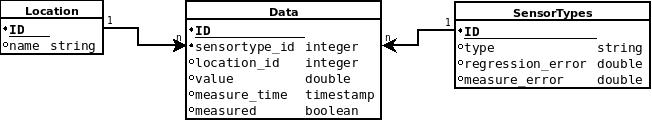
\includegraphics[scale=0.6]{4/figures/data_model_final.jpg}
\caption{Updated Server-side Data Model}
\label{data_model_final}
\end{figure}

\subsection{Simple Linear Regression}

A simple linear regression model was selected to predict future data, which uses the least squares method to calculate the future values. \todo{add a mention of the paper the idea was taken from?} The model has a single explanatory variable - Unix time. This variable is used to predict the future values of sensor readings based on previous measurements. 

The model sample is taken from previous measurements during the last \todo{actual time} 5 minutes. The 5 minute interval is selected to balance out errors caused by extreme values. This is necessary because a single value with big enough deviation can cause the regression model to become inaccurate. 

To measure the accuracy of the model, an confidence level of 90\% was introduced. If the sample for last 5 minutes provides an accurate enough regression model, then the predictions can be used. Otherwise, fresh data should be queried and added to the model until the error threshold is satisfied. The equation to calculate regression model's confidence level $\alpha$:\\

\begin{center}
$\alpha = 2\Phi \left ( \frac{\epsilon}{RMSE}  \right ) - 1$.
\end{center}

Here $\Phi$ is the CDF (Cumulative Distribution Function) of residuals, $\epsilon$ is the allowed error (in the database model named as $regression\_error$ and $RMSE$ is the root mean square error the regression model. \todo{maybe describe what rmse is?}

Regression models are created separately for each sensor. Each model has a sample of previous measurements and the allowed error $\epsilon$ defined in the database. 
The confidence level $\alpha$ is calculated for each model and has to be over $90\%$ which is the selected confidence threshold. If all regression models satisfy the confidence level, then the fuzzy control system is initialized with data from previous measurements and calculated confidence levels. 

\subsection{Fuzzy Logic Engine}

The next step in predicting future sensor values is to calculate the time interval for the next measurement request. To calculate the time, a fuzzy control system was introduced to provide flexible decisions based on multiple input variables. The input variables are: 
\begin{enumerate}
\item $temp$					
\item $temp$ $predictability$	
\item $light$					
\item $light$ $predictability$	
\item $hall$					
\item $hall$ $predictability$
\end{enumerate}

Here each sensor has a pair of input variables - measured sensor value and sensor value predictability (regression model confidence level $\alpha$). All these variables are mapped into fuzzy sets, a procedure call fuzzification. The predictability variables are mapped into sets which all have the same membership functions shown in figure \autoref{pred_sets}.

\begin{figure}[h!]
\centering
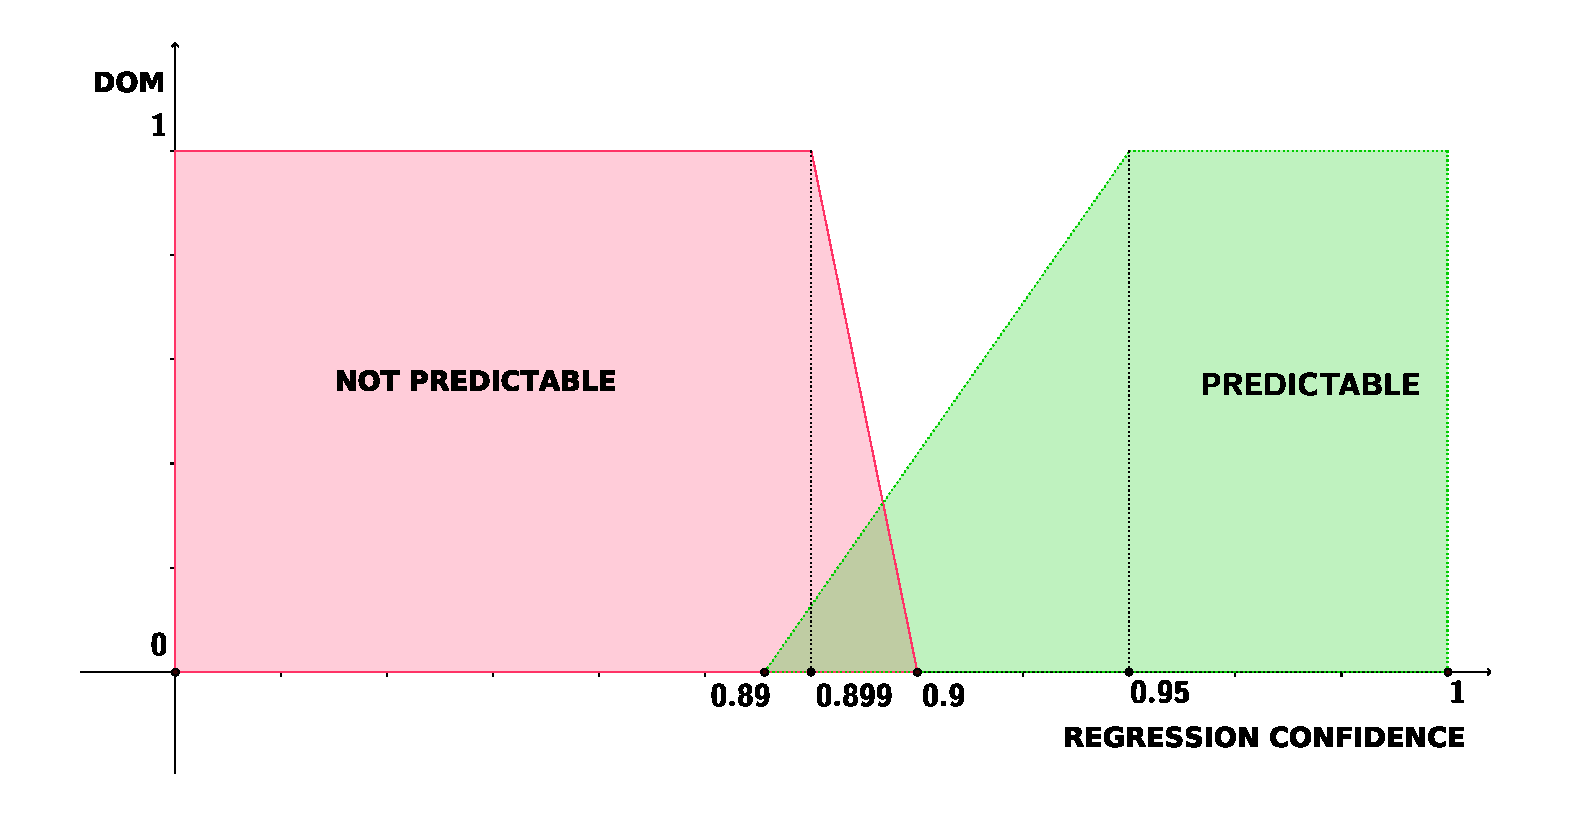
\includegraphics[scale=0.58]{4/figures/pred_sets.pdf}
\caption{Regression Confidence Fuzzy Sets}
\label{pred_sets}
\end{figure}

The fuzzy control system is initialized with a previous measurement for each sensor. This effectively sets the bounds of each sensor's fuzzy sets as seen in \autoref{change_sets}. The $PREDICTABLE$ fuzzy set's DOM (degree of membership) reaches maximum at a confidence level of 0.95 or 95\% because for our prototype anything above that level is highly predictable. 

The measured sensor values are fuzzified into sets, which each have different membership functions. The membership functions are calculated on the last measurement received as seen in \autoref{change_sets}. Here $X$ in set labels notes the sensor type currently used as the sets are the same relative to each sensor's previous measurement. The center point $O$ is the previously measured value. $||X_2X_3||$ is the predefined sensor measurement error  ($sensor\_error$ field in the data model). This means that if the new measurement is between the points $X_2$ and $X_3$, there is no change in the measurement for the fuzzy system. The lengths $||X_0X_2||$, $||X_1O||$, $||OX_4||$ and $||X_3X_5||$ are defined by the same variable $slope\_width$. \todo{maybe calculate this automatically somehow, atm predefined variable used}

\begin{figure}[h!]
\centering
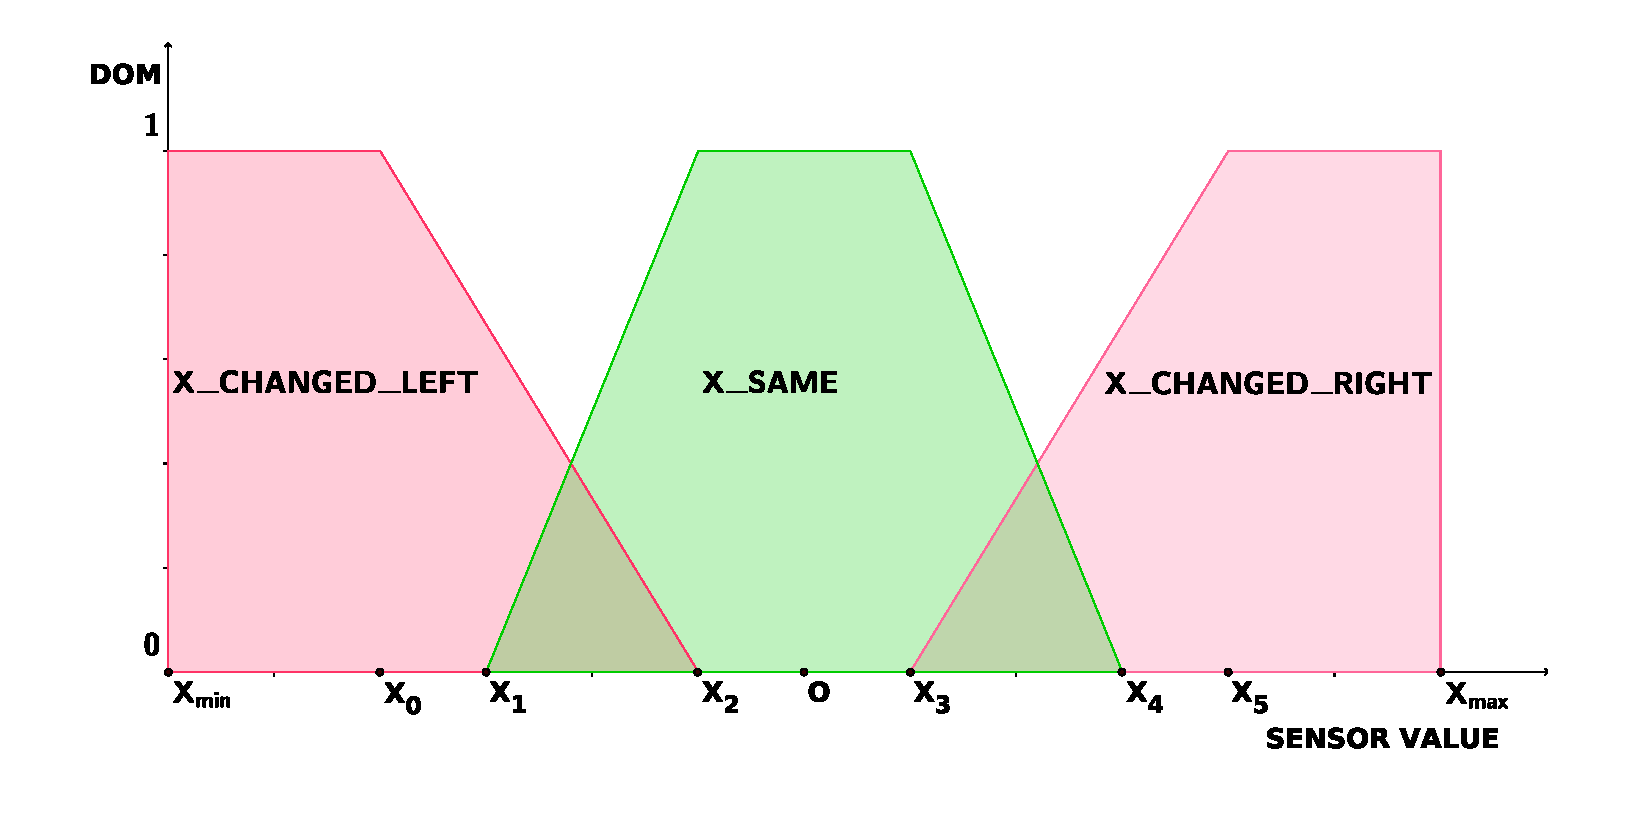
\includegraphics[scale=0.55]{4/figures/change_sets.pdf}
\caption{Sensor Value Fuzzy Sets}
\label{change_sets}
\end{figure}

\todo{Add a table with the selected error values for fuzzy engine and prediction here}

The output variable is defuzzified from the idle time sets which have membership functions described in \autoref{idle_sets}. The sets $request$ and $predict$ are symmetrical to enable easy defuzzification. The maximum idle time is 65 seconds, which is the maximum length of one sleep cycle for the sensor module. 

\begin{figure}[h!]
\centering
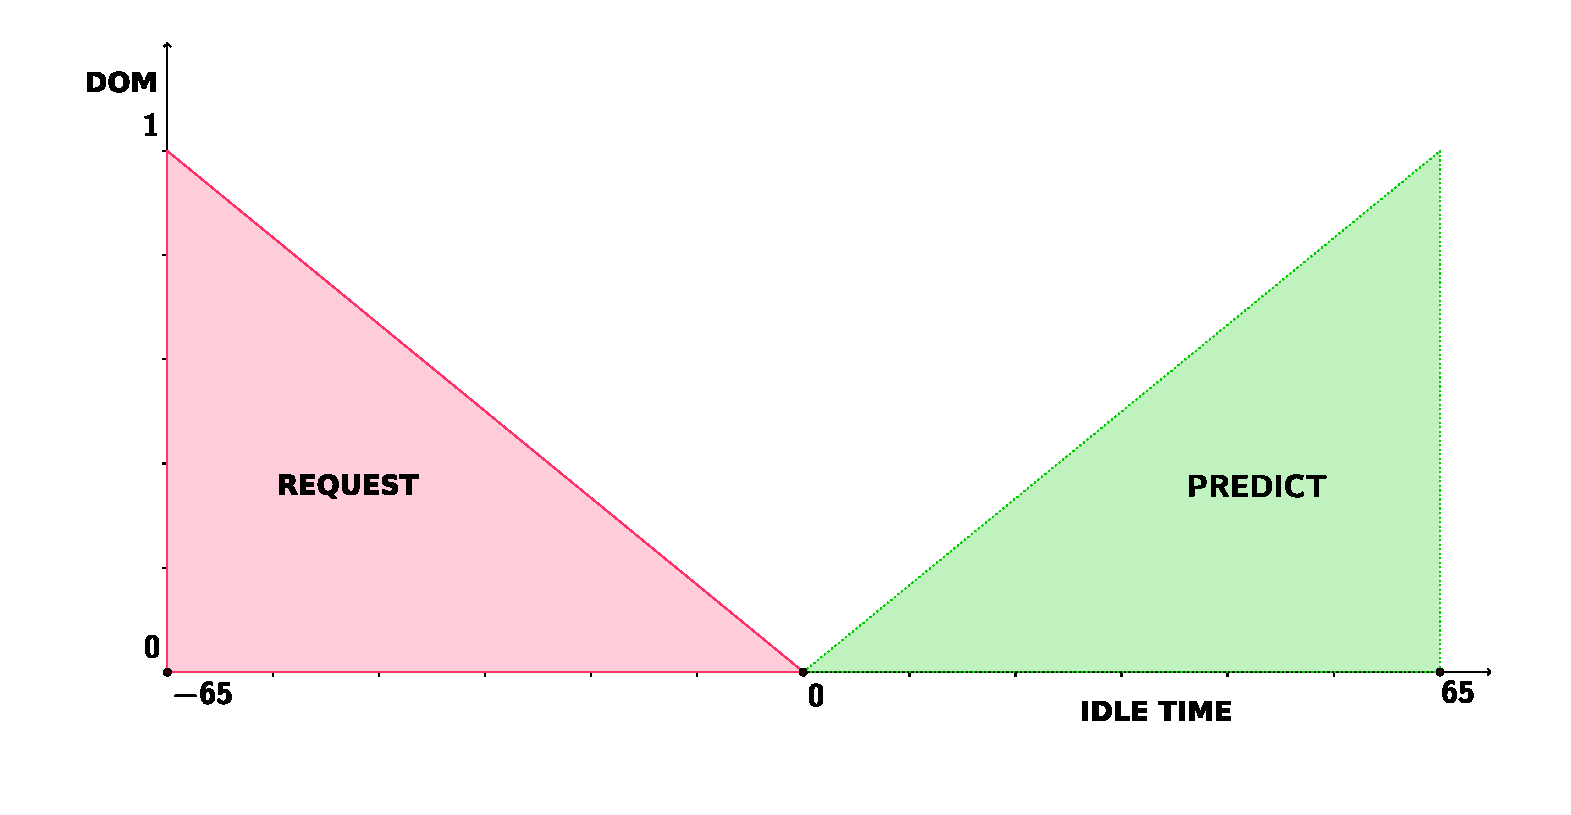
\includegraphics[scale=0.58]{4/figures/result_sets.pdf}
\caption{Idle Time Fuzzy Sets}
\label{idle_sets}
\end{figure}

When all input variables have been fuzzified and degrees of membership calculated, then the next step is to fire all predefined rules. For each sensor, there is a collection of 3 rules, making a total of 9 rules (here $x \in \{hall, temp, light\}$):

\begin{enumerate}
\item IF $x$ IS $x\_changed\_left$ OR $x\_changed\_right$ AND $x\_predictability$ IS $not\_predictable$ OR $predictable$ THEN $request$
\item IF $x$ IS $x\_same$ AND $x\_predictability$ IS $not\_predictable$ THEN $request$
\item IF $x$ IS $x\_same$ AND $x\_predictability$ IS $predictable$ THEN $predict$
\end{enumerate}

The previously calculated degrees of membership are fed into these rules. For $AND$ relationship, the minimum value is selected, for $OR$ relationship, the maximum value is selected. For each rule, the output variable received a DOM equal to the DOM of the premise. When all rules have been evaluated, the results are defuzzified into a single crisp value, which is the idle time decision. This process is called defuzzification.

During defuzzification the DOMs of result sets $request$ and $predict$ for each rule are combined into a single DOM for the specified set. For this, $request$ output has an $OR$ relationship (maximum value) and the $predict$ set has an $AND$ relationship (minimum value). These relationships mean that the most inaccurate sensors would be represented in the final result. For example if $hall$ has a DOM of 1.0 to $predict$, but $temp$ has a DOM of 0.5 to $predict$, then the outcome would be a DOM of 0.5, because we need the output for least accurate sensors. For $request$ this logic is reversed as the maximum DOM to $request$ represents the output for the least accurate sensor. 

The next step is to get the crisp result value. For this process, the idle time values for $predict$ and $request$ set membership functions at the specified DOM are calculated. $x$ is found the equation $f(x) = DOM$, where $x$ is the idle time and $f$ is the membership function. $request$ and $predict$ membership functions are symmetric with the axis being in the point $x = 0$ as seen in \autoref{idle_sets}. The final defuzzified idle time is equal to $max\{x_{predict} - x_{request}, 10\}$. Meaning that if the DOM to $request$ was higher that to predict, then the default idle time of 10 seconds is returned. Otherwise the value at the center point of the two results is returned.

When the crisp result is received from the fuzzy control system and idle time is longer than 10 seconds, future data is predicted for the idle period. This means that using the regression models, future values with 10 second intervals are inserted into the database for each sensor. 

Finally, the idle time with a minimum value of 10 seconds is written as a JSON format string to the response body of the HTTP request. A sample response would look like:\\ \todo{add a sample response here}

\begin{lstlisting}
HTTP/1.1 200 OK
Content-Type: application/json;charset=utf-8
Content-Length: 12
Connection: close
Server: Jetty(7.2.0.v20101020)

{"idle": 34}
\end{lstlisting}

\section{Results}
\todo{Describe tests carried out}\\
\todo{Make a test with a 9V battery}\\
\todo{Graphs with improved power consumption figures on it, description of what changed and how/why}
\todo{Graph with 10s idle time as the worst-case scenario here}

% ---------------------------------------------------------------------------
%: ----------------------- end of thesis sub-document ------------------------
% ---------------------------------------------------------------------------

